\SourcePage{151}{154}
\section{Motion in a Coulomb field (spherical coordinates)}

An especially important case of motion in a central field is motion in a
\emph{Coulomb field},
\[U=\pm\frac\alpha r,\]
where $\alpha>0$. We first consider attraction and write $U=-\alpha/r$.
General considerations already show that the negative-energy spectrum is
discrete, with infinitely many levels, whereas the positive-energy spectrum
is continuous.

Equation (32.8) for the radial functions becomes
\begin{equation}
 \frac{d^2R}{dr^2}+\frac2r\frac{dR}{dr}-\frac{l(l+1)}{r^2}R
 +\frac{2m}{\hbar^2}\left(E+\frac\alpha r\right)R=0. \tag{36.1}
\end{equation}

For the relative motion of two attracting particles, $m$ denotes their
reduced mass.

Calculations in a Coulomb field are conveniently made in special
\emph{Coulomb units}. We choose as the units of mass, length, and time
\[m,\qquad \frac{\hbar^2}{m\alpha},\qquad\frac{\hbar^3}{m\alpha^2}.\]
All other units follow; the energy unit is $m\alpha^2/\hbar^2$. These units
are used throughout this and the next section unless stated otherwise.\footnote{For an electron of mass $m=9.11\cdot10^{-28}$ g and $\alpha=e^2$,
the Coulomb units coincide with the \emph{atomic units}. The atomic length
unit is $\hbar^2/me^2=0.529\cdot10^{-8}\ \text{cm}$, the \emph{Bohr radius}.
The atomic energy unit is
$me^4/\hbar^2=4.36\cdot10^{-11}\ \text{erg}=27.21\ \text{eV}$; half of it is
the \emph{rydberg}, Ry. The atomic charge unit is
$e=4.80\cdot10^{-10}$ electrostatic units. Formally, formulas are converted
to atomic units by putting $e=m=\hbar=1$. For $\alpha=Ze^2$, Coulomb and
atomic units differ.}
\SourcePage{152}{155}
In these units (36.1) is
\begin{equation}
 \frac{d^2R}{dr^2}+\frac2r\frac{dR}{dr}-\frac{l(l+1)}{r^2}R
 +2\left(E+\frac1r\right)R=0. \tag{36.2}
\end{equation}

\textbf{Discrete spectrum.} Introduce
\begin{equation}n=\frac1{\sqrt{-2E}},\qquad\rho=\frac{2r}{n}.\tag{36.3}\end{equation}
For negative energy $n$ is real and positive. Equation (36.2) becomes
\begin{equation}
 R''+\frac2\rho R'+\left[-\frac14+\frac n\rho-\frac{l(l+1)}{\rho^2}\right]R=0,
 \tag{36.4}
\end{equation}
where primes mean differentiation with respect to $\rho$.

At small $\rho$ the admissible solution is proportional to $\rho^l$ (see
(32.15)). At large $\rho$, omission of the $1/\rho$ and $1/\rho^2$ terms
gives $R''=R/4$, hence $R=e^{\pm\rho/2}$. The solution vanishing at infinity
therefore behaves as $e^{-\rho/2}$. Put
\begin{equation}R=\rho^le^{-\rho/2}\omega(\rho).\tag{36.5}\end{equation}
Then
\begin{equation}
 \rho\omega''+(2l+2-\rho)\omega'+(n-l-1)\omega=0. \tag{36.6}
\end{equation}
The solution must grow no faster than a finite power at infinity and remain
finite at the origin.
\SourcePage{153}{156}
The solution satisfying the latter condition is the confluent hypergeometric
function
\begin{equation}\omega=F(-n+l+1,2l+2,\rho)\tag{36.7}\end{equation}
(see mathematical appendix \S~d).\footnote{The second solution of (36.6)
diverges as $\rho^{-2l-1}$ when $\rho\to0$.} The condition at infinity holds
only when $-n+l+1$ is a nonpositive integer, so that (36.7) is a polynomial
of degree $n-l-1$; otherwise it grows as $e^\rho$ (see (d.14)). Thus $n$ is a
positive integer and
\begin{equation}n\geq l+1.\tag{36.8}\end{equation}
From (36.3),
\begin{equation}E=-\frac1{2n^2},\qquad n=1,2,\ldots.\tag{36.9}\end{equation}

This determines the discrete energy levels. Infinitely many lie between the
normal level $E_1=-1/2$ and zero. Their spacings decrease with $n$, and they
accumulate at $E=0$, where the discrete and continuous spectra meet. In
ordinary units,\footnote{Formula (36.10) was first obtained by N.~Bohr in
1913, before quantum mechanics. W.~Pauli derived it in quantum mechanics by
the matrix method in 1926, and Schrödinger derived it from the wave equation
a few months later.}
\begin{equation}E=-\frac{m\alpha^2}{2\hbar^2n^2}.\tag{36.10}\end{equation}

The integer $n$ is the \emph{principal quantum number}; the radial quantum
number of \secref{32} is $n_r=n-l-1$. At fixed $n$,
\begin{equation}l=0,1,\ldots,n-1.\tag{36.11}\end{equation}
Since the energy depends only on $n$, states with different $l$ but the same
$n$ have equal energies.
\SourcePage{154}{157}
Each eigenvalue is therefore degenerate not only in the magnetic quantum
number $m$, as in every central field, but also in $l$. This latter,
\emph{accidental} or \emph{Coulomb}, degeneracy is peculiar to the Coulomb
field. Since each $l$ has $2l+1$ values of $m$, the degeneracy of level $n$ is
\begin{equation}\sum_{l=0}^{n-1}(2l+1)=n^2.\tag{36.12}\end{equation}

The stationary-state wave functions follow from (36.5) and (36.7). For
integer parameters the confluent hypergeometric function is, apart from a
factor, a generalized Laguerre polynomial (appendix \S~d), so
\[R_{nl}=\operatorname{const}\cdot\rho^le^{-\rho/2}L_{n+l}^{2l+1}(\rho).\]
With $\int_0^\infty R_{nl}^2r^2\,dr=1$, the final form is\footnote{The first
few functions are
\[
\begin{gathered}
R_{10}=2e^{-r},\quad R_{20}=\frac1{\sqrt2}e^{-r/2}(1-r/2),\quad
R_{21}=\frac1{2\sqrt6}e^{-r/2}r,\\
R_{30}=\frac2{3\sqrt3}e^{-r/3}(1-2r/3+2r^2/27),\\
R_{31}=\frac8{27\sqrt6}e^{-r/3}r(1-r/6),\quad
R_{32}=\frac4{81\sqrt{30}}e^{-r/3}r^2.
\end{gathered}
\]}
\begin{equation}
\begin{aligned}
R_{nl}&=-\frac2{n^2}\sqrt{\frac{(n-l-1)!}{[(n+l)!]^3}}e^{-r/n}
 (2r/n)^lL_{n+l}^{2l+1}(2r/n)\\
&=\frac2{n^{l+2}(2l+1)!}\sqrt{\frac{(n+l)!}{(n-l-1)!}}
 (2r)^le^{-r/n}F(-n+l+1,2l+2,2r/n).
\end{aligned}\tag{36.13}
\end{equation}
\SourcePage{155}{158}
(For the normalization integral see appendix \S~f, integral (f.6).\footnote{It
may also be evaluated by substituting (d.13) for the Laguerre polynomials and
integrating by parts, as for the Legendre-polynomial integral (c.8).}) Near
the origin,
\begin{equation}
 R_{nl}\approx r^l\frac{2^{l+1}}{n^{2+l}(2l+1)!}
 \sqrt{\frac{(n+l)!}{(n-l-1)!}}.\tag{36.14}
\end{equation}
At large distances,
\begin{equation}
 R_{nl}\approx(-1)^{n-l-1}\frac{2^n r^{n-1}e^{-r/n}}
 {n^{n+1}\sqrt{(n+l)!(n-l-1)!}}.\tag{36.15}
\end{equation}
The normal-state function $R_{10}$ decays over distances $r\sim1$, or
$r\sim\hbar^2/m\alpha$ in ordinary units.

Mean powers of $r$ are $\overline{r^k}=\int_0^\infty r^{k+2}R_{nl}^2dr$.
The general result follows from (f.7); some first values are
\begin{equation}
\begin{gathered}
\bar r=\tfrac12[3n^2-l(l+1)],\qquad
\overline{r^2}=\tfrac{n^2}{2}[5n^2+1-3l(l+1)],\\
\overline{r^{-1}}=\frac1{n^2},\qquad
\overline{r^{-2}}=\frac1{n^3(l+1/2)}.
\end{gathered}\tag{36.16}
\end{equation}

\textbf{Continuous spectrum.} Positive energies form a continuous spectrum
from zero to infinity. Every eigenvalue is infinitely degenerate, with all
integer $l\geq0$ and all allowed $m$. Now $n$ and $\rho$ are purely imaginary:
\begin{equation}n=-\frac i{\sqrt{2E}}=-\frac ik,\qquad\rho=2ikr,\tag{36.17}\end{equation}
\SourcePage{156}{159}
where $k=\sqrt{2E}$.\footnote{One could instead choose the complex conjugates
$n=i/k$, $\rho=-2ikr$; the real functions $R_{kl}$ are independent of this
choice.} The continuum radial eigenfunctions are
\begin{equation}
 R_{kl}=\frac{C_{kl}}{(2l+1)!}(2kr)^le^{-ikr}
 F(i/k+l+1,2l+2,2ikr),\tag{36.18}
\end{equation}
or, as a complex integral (appendix \S~d),
\begin{equation}
 R_{kl}=C_{kl}(2kr)^le^{-ikr}\frac1{2\pi i}\oint
 e^\xi\left(1-\frac{2ikr}{\xi}\right)^{-i/k-l-1}\xi^{-2l-2}d\xi,
 \tag{36.19}
\end{equation}
over the contour in Fig.~10.\footnote{It may be replaced by any closed loop
encircling $\xi=0$ and $\xi=2ikr$ positively. For integral $l$, the function
$V(\xi)=\xi^{-n-l}(\xi-2ikr)^{n-l}$ (appendix \S~d) returns to its original
value around such a contour.} With $\xi=2ikr(t+1/2)$ this becomes
\begin{equation}
 R_{kl}=C_{kl}\frac{(-2kr)^{-l-1}}{2\pi}\oint e^{2ikrt}
 (t+\tfrac12)^{i/k-l-1}(t-\tfrac12)^{-i/k-l-1}dt.\tag{36.20}
\end{equation}
The path encircles $t=\pm1/2$ positively; this form directly shows that
$R_{kl}$ is real.

\begin{center}
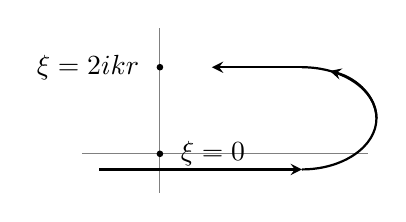
\begin{tikzpicture}[x=2.2cm,y=1.1cm,>=stealth]
 \draw[gray] (-0.45,0)--(1.2,0); \draw[gray] (0,-0.45)--(0,1.45);
 \fill (0,0) circle (1.2pt) node[right=4pt] {$\xi=0$};
 \fill (0,1) circle (1.2pt) node[left=4pt] {$\xi=2ikr$};
 \draw[thick,->] (-0.35,-0.18)--(0.82,-0.18);
 \draw[thick] (0.82,-0.18) arc (-90:90:0.43 and 0.59);
 \draw[thick,->] (1.25,0.41) arc (0:68:0.43 and 0.59);
 \draw[thick,->] (0.82,1)--(0.3,1);
\end{tikzpicture}

\small Fig.~10
\end{center}

Using (d.14), the asymptotic expansion is
\begin{equation}
\begin{aligned}
R_{kl}=C_{kl}\frac{e^{-\pi/2k}}{kr}\operatorname{Re}\Biggl\{&
\frac{\exp[-i(kr-(\pi/2)(l+1)+(1/k)\ln2kr)]}{\Gamma(l+1-i/k)}\\[-2pt]
&\times G(l+1+i/k,i/k-l,-2ikr)\Biggr\}.
\end{aligned}\tag{36.21}
\end{equation}
For normalization on the $k/2\pi$ scale, condition (33.4),
\begin{equation}C_{kl}=2ke^{\pi/2k}|\Gamma(l+1-i/k)|.\tag{36.22}\end{equation}
\SourcePage{157}{160}
Indeed, at large $r$ this gives
\begin{equation}
 R_{kl}\approx\frac2r\sin(kr+k^{-1}\ln2kr-\pi l/2+\delta_l),\qquad
 \delta_l=\arg\Gamma(l+1-i/k).\tag{36.23}
\end{equation}
This agrees with the general form (33.20), apart from the logarithmic phase;
since $\ln r$ grows slowly compared with $r$, it does not affect the divergent
normalization integral.

The gamma-function modulus in (36.22) is elementary. From
$\Gamma(z+1)=z\Gamma(z)$ and
$\Gamma(z)\Gamma(1-z)=\pi/\sin\pi z$, one finds
\[
\begin{aligned}
\Gamma(l+1+i/k)&=(l+i/k)\cdots(1+i/k)(i/k)\Gamma(i/k),\\
\Gamma(l+1-i/k)&=(l-i/k)\cdots(1-i/k)\Gamma(1-i/k),
\end{aligned}
\]
and
\[
|\Gamma(l+1-i/k)|=\sqrt{\frac\pi k}\prod_{s=1}^l\sqrt{s^2+k^{-2}}
(\sinh(\pi/k))^{-1/2}.
\]
Thus
\begin{equation}
 C_{kl}=\left[\frac{8\pi k}{1-e^{-2\pi/k}}\right]^{1/2}
 \prod_{s=1}^{l}\sqrt{s^2+\frac1{k^2}},\tag{36.24}
\end{equation}
with the product replaced by 1 at $l=0$.
\SourcePage{158}{161}
The $E=0$ radial function follows by taking $k\to0$:
\[
\begin{aligned}
F(i/k+l+1,2l+2,2ikr)&\to F(i/k,2l+2,2ikr)\\
&=1-\frac{2r}{(2l+1)!}+\frac{(2r)^2}{(2l+2)(2l+3)2!}-\cdots\\
&=(2l+1)!(2r)^{-l-1/2}J_{2l+1}(\sqrt{8r}),
\end{aligned}
\]
where $J_{2l+1}$ is a Bessel function, while
$C_{kl}\approx\sqrt{8\pi}\,k^{-l+1/2}$. Hence
\begin{equation}
 \left.\frac{R_{kl}}{\sqrt k}\right|_{k\to0}
 =\sqrt{\frac{4\pi}{r}}J_{2l+1}(\sqrt{8r}).\tag{36.25}
\end{equation}
At large $r$,\footnote{This function corresponds to the semiclassical
approximation (\secref{49}) in $(l+1/2)^2\ll r\ll k^{-2}$.}
\begin{equation}
 \left.\frac{R_{kl}}{\sqrt k}\right|_{k\to0}
 =\left(\frac8{r^3}\right)^{1/4}\sin(\sqrt{8r}-l\pi-\pi/4).\tag{36.26}
\end{equation}
The factor $\sqrt k$ disappears on changing to energy-scale normalization,
from $R_{kl}$ to $R_{El}$ by (33.5); $R_{El}$ remains finite as $E\to0$.

For the repulsive field $U=\alpha/r$, only a continuous positive-energy
spectrum exists. Formally changing $r$ to $-r$ in the attractive-field
equation gives
\begin{equation}
\begin{gathered}
 R_{kl}=\frac{C_{kl}}{(2l+1)!}(2kr)^le^{ikr}F(i/k+l+1,2l+2,-2ikr),\\
 C_{kl}=2ke^{-\pi/2k}|\Gamma(l+1+i/k)|
 =\left(\frac{8\pi k}{e^{2\pi/k}-1}\right)^{1/2}
 \prod_{s=1}^{l}\sqrt{s^2+\frac1{k^2}}.
\end{gathered}\tag{36.27}
\end{equation}
\SourcePage{159}{162}
At large $r$,
\begin{equation}
 R_{kl}\approx\frac2r\sin(kr-k^{-1}\ln2kr-l\pi/2+\delta_l),\qquad
 \delta_l=\arg\Gamma(l+1+i/k).\tag{36.28}
\end{equation}
\textbf{Origin of the Coulomb degeneracy.} Classical motion in an attractive
Coulomb field has the special conserved quantity
\begin{equation}
 \mathbf A=\frac{\mathbf r}{r}-\mathbf p\times\mathbf l=\operatorname{const}
 \tag{36.29}
\end{equation}
(see I, \S~15). Its quantum operator is
\begin{equation}
 \hat{\mathbf A}=\frac{\mathbf r}{r}-\frac12
 (\hat{\mathbf p}\times\hat{\mathbf l}-\hat{\mathbf l}\times\hat{\mathbf p}),
 \tag{36.30}
\end{equation}
which commutes with $\hat H=\hat{\mathbf p}^{2}/2-1/r$.

Direct calculation gives
\begin{equation}
 [\hat l_i,\hat A_k]=i e_{ikl}\hat A_l,\qquad
 [\hat A_i,\hat A_k]=-2i\hat H e_{ikl}\hat l_l.\tag{36.31}
\end{equation}
The mutual noncommutativity of the $\hat A_i$ means that $A_x,A_y,A_z$
cannot all be definite. Each component, say $\hat A_z$, commutes with
$\hat l_z$ but not with $\hat{\mathbf l}^{2}$. A new conserved quantity
which cannot be measured together with the other conserved quantities causes
the additional degeneracy (\secref{10}): this is the accidental degeneracy peculiar
to the Coulomb field.

The same origin may be stated in terms of the Coulomb problem's enlarged
quantum-mechanical symmetry (V.~A. Fock, 1935). At fixed negative energy,
replace $\hat H$ on the right of (36.31) by $E$ and define
$\hat u_i=\hat A_i/\sqrt{-2E}$. Then
\SourcePage{160}{163}
\begin{equation}
 [\hat l_i,\hat u_k]=i e_{ikl}\hat u_l,\qquad
 [\hat u_i,\hat u_k]=i e_{ikl}\hat l_l.\tag{36.32}
\end{equation}
Together with $[\hat l_i,\hat l_k]=i e_{ikl}\hat l_l$, these are precisely the
formal commutation rules for infinitesimal rotations in four-dimensional
Euclidean space.\footnote{Here $\hat l_x,\hat l_y,\hat l_z$ generate rotations
in the $yz,xz,xy$ planes of Cartesian coordinates $x,y,z,u$, and
$\hat u_x,\hat u_y,\hat u_z$ generate rotations in the $xu,yu,zu$ planes.}
This is the symmetry of the Coulomb problem.\footnote{It appears explicitly
in momentum-space wave functions; see V.~A. Fock, Izv. AN SSSR, physical
series, 1935, no.~2, p.~169; Zs. f. Physik 98 (1935), 145.}

The energy levels can again be derived from (36.32).\footnote{This derivation
is essentially Pauli's (1926).} Introduce
\begin{equation}
 \hat{\mathbf j}_1=\tfrac12(\hat{\mathbf l}+\hat{\mathbf u}),\qquad
 \hat{\mathbf j}_2=\tfrac12(\hat{\mathbf l}-\hat{\mathbf u}).\tag{36.33}
\end{equation}
Then
\begin{equation}
 [\hat j_{1i},\hat j_{1k}]=ie_{ikl}\hat j_{1l},\quad
 [\hat j_{2i},\hat j_{2k}]=ie_{ikl}\hat j_{2l},\quad
 [\hat j_{1i},\hat j_{2k}]=0.\tag{36.34}
\end{equation}
These are the rules for two independent three-dimensional angular momenta.
Thus the eigenvalues of $\hat{\mathbf j}_1^{2}$ and
$\hat{\mathbf j}_2^{2}$ are $j_1(j_1+1)$ and $j_2(j_2+1)$, with
$j_1,j_2=0,1/2,1,3/2,\ldots$.\footnote{We anticipate \secref{54} in using the
possible integral and half-integral values of $j$.} Directly from
$\hat{\mathbf u}$ and $\hat{\mathbf l}=\mathbf r\times\hat{\mathbf p}$,
\[
 \hat{\mathbf l}\hat{\mathbf u}=\hat{\mathbf u}\hat{\mathbf l}=0,
 \qquad \hat{\mathbf l}^{2}+\hat{\mathbf u}^{2}=-1-\frac1{2E}
 \qquad \hat{\mathbf l}^{2}+\hat{\mathbf u}^{2}=-1-\frac1{2E}.
\]
Hence
\[
 \hat{\mathbf j}_1^{2}=\hat{\mathbf j}_2^{2}
 =-\tfrac14(1+1/2E)=j(j+1),
\]
so $E=-1/[2(2j+1)^2]$. Writing
\begin{equation}2j+1=n,\qquad n=1,2,3,\ldots,\tag{36.35}\end{equation}
\SourcePage{161}{164}
gives $E=-1/(2n^2)$. The degeneracy is
$(2j_1+1)(2j_2+1)=n^2$. Since
$\hat{\mathbf l}=\hat{\mathbf j}_1+\hat{\mathbf j}_2$, for
$j_1=j_2=(n-1)/2$ the orbital momentum ranges from $l=0$ to $2j=n-1$.\footnote{Accidental degeneracy between different $l$ also occurs in the
central field $U=m\omega^2r^2/2$ (the spatial oscillator; Problem 4 of
\secref{33}), again because of an enlarged Hamiltonian symmetry. In
$\hat H=\hat{\mathbf p}^{2}/2m+m\omega^2r^2/2$, both $\hat p_i$ and $x_i$
enter as sums of squares. With
\[
 \hat a_i=\frac{m\omega x_i+i\hat p_i}{\sqrt{2m\hbar\omega}},\qquad
 \hat a_i^+=\frac{m\omega x_i-i\hat p_i}{\sqrt{2m\hbar\omega}},
\]
one obtains
$\hat H=\hbar\omega[\hat{\mathbf a}^{+}\hat{\mathbf a}+3/2]$.
This is invariant under arbitrary unitary transformations of $\hat a_i^+$
and $\hat a_j$, a group larger than the three-dimensional rotation group.
The quantum peculiarity of the Coulomb and oscillator fields has its classical
counterpart: particle trajectories are closed in these, and only these,
fields.}

\ProblemHeading

\textbf{1.} Find the probability distribution of momentum values in the
ground state of the hydrogen atom.

\SolutionHeading\footnote{Atomic units are used in Problems 1 and 2.} The
ground-state wave function is
\[\psi=R_{10}Y_{00}=\frac1{\sqrt\pi}e^{-r}.\]
In the $\mathbf p$-representation,
\[a(\mathbf p)=\int\psi(\mathbf r)e^{-i\mathbf p\mathbf r}\,dV.\]
Using spherical coordinates with polar axis along $\mathbf p$ gives
\[a(\mathbf p)=\frac{8\sqrt\pi}{(1+p^2)^2},\]
and the probability density in momentum space is
$|a(\mathbf p)|^2/(2\pi)^3$.

\textbf{2.} Find the mean potential of the field produced by the nucleus and
the electron in the hydrogen ground state.
\SourcePage{162}{165}
\SolutionHeading The mean potential $\varphi_e$ of the ``electron cloud'' is
most simply found as the spherical solution of Poisson's equation with charge
density $\rho=-|\psi|^2$:
\[\frac1r\frac{d^2}{dr^2}(r\varphi_e)=4e^{-2r}.\]
Choosing the integration constants so that $\varphi_e(0)$ is finite and
$\varphi_e(\infty)=0$, and adding the nuclear potential, gives
\[\varphi=1/r+\varphi_e(r)=(1/r+1)e^{-2r}.\]
Thus $\varphi\approx1/r$ for $r\ll1$, while
$\varphi\approx e^{-2r}$ for $r\gg1$.

\newpage
\textbf{3.} Find the energy levels of a particle moving in the central field
$U=A/r^2-B/r$ (Fig.~11).

\begin{center}
\begin{tikzpicture}[x=1.2cm,y=0.8cm,>=stealth]
 \draw[->] (0,-2.1)--(0,2.2) node[above] {$U(r)$};
 \draw[->] (0,0)--(4,0) node[right] {$r$};
 \draw[thick,domain=0.28:4,samples=100,smooth]
   plot (\x,{1.1/(\x*\x)-1.65/\x});
\end{tikzpicture}

\small Fig.~11
\end{center}

\SolutionHeading Positive energies form a continuous spectrum and negative
energies a discrete one; consider the latter. The radial equation is
\begin{equation}
 \frac{d^2R}{dr^2}+\frac2r\frac{dR}{dr}+\frac{2m}{\hbar^2}
 \left(E-\frac{\hbar^2l(l+1)}{2mr^2}-\frac A{r^2}+\frac Br\right)R=0.
 \tag{1}
\end{equation}
Put $\rho=2\sqrt{-mE}\,r/\hbar$ and define
\begin{equation}\frac{2mA}{\hbar^2}+l(l+1)=s(s+1),\tag{2}\end{equation}
\begin{equation}\frac B\hbar\sqrt{\frac m{-2E}}=n.\tag{3}\end{equation}
Then
\[R''+\frac2\rho R'+(-\tfrac14+n/\rho-s(s+1)/\rho^2)R=0,\]
formally identical to (36.4). Hence
\[R=\rho^se^{-\rho/2}F(-n+s+1,2s+2,\rho),\]
where $n-s-1=p$ is a nonnegative integer and $s$ is the positive root of
(2). Formula (3) gives
\[
 -E_p=\frac{2B^2m}{\hbar^2}
 [2p+1+\sqrt{(2l+1)^2+8mA/\hbar^2}]^{-2}.
\]

\textbf{4.} Repeat the calculation for $U=A/r^2+Br^2$ (Fig.~12).

\SolutionHeading There is only a discrete spectrum. The radial equation is
\[
 \frac{d^2R}{dr^2}+\frac2r\frac{dR}{dr}+\frac{2m}{\hbar^2}
 (E-\hbar^2l(l+1)/(2mr^2)-A/r^2-Br^2)R=0.
\]
\SourcePage{163}{166}
Set
\[\xi=\frac{\sqrt{2mB}}\hbar r^2,\]
and define
\[l(l+1)+\frac{2mA}{\hbar^2}=2s(2s+1),\qquad
 \sqrt{\frac{2m}{B}}\frac E\hbar=4(n+s)+3.\]
Then
\[
 \xi R''+\frac32R'+[n+s+\tfrac34-\xi/4-s(s+1/2)/\xi]R=0.
\]
The desired solution behaves as $e^{-\xi/2}$ at infinity and as $\xi^s$ at
the origin, where
\[s=\frac14[-1+\sqrt{(2l+1)^2+8mA/\hbar^2}].\]

\begin{center}
\begin{tikzpicture}[x=1.2cm,y=0.8cm,>=stealth]
 \draw[->] (0,-0.8)--(0,3.2) node[above] {$U(r)$};
 \draw[->] (0,0)--(4,0) node[right] {$r$};
 \draw[thick,domain=0.3:3.7,samples=100,smooth]
   plot (\x,{0.55/(\x*\x)+0.26*\x*\x-1.05});
\end{tikzpicture}

\small Fig.~12
\end{center}

Writing $R=e^{-\xi/2}\xi^s\omega$ gives
\[\xi\omega''+(2s+3/2-\xi)\omega'+n\omega=0,\]
so
\[\omega=F(-n,2s+3/2,\xi),\]
where $n$ is a nonnegative integer. The equally spaced levels are
\[
 E_n=\hbar\sqrt{\frac B{2m}}
 [4n+2+\sqrt{(2l+1)^2+8mA/\hbar^2}],\qquad n=0,1,2,\ldots.
\]

